\documentclass{article}
\usepackage{hyperref}
\usepackage{amsmath,amssymb}
\usepackage{graphicx}
\usepackage{caption}
\usepackage{subcaption}
\usepackage{color}
\usepackage[section]{placeins}
\renewcommand{\thesubsection}{\thesection.\alph{subsection}}
\usepackage{listings}

\newcommand{\abs}[1]{\ensuremath{ \left|#1\right|}}
\newcommand{\norm}[1]{\ensuremath{ \left|\left|#1\right|\right|}}
\newcommand{\orderof}[1]{\ensuremath{ {\cal O}\left(#1\right)}}
\newcommand{\pdv}[2]{\frac{\partial #1}{\partial #2}}
\newcommand{\grad}[1]{\bv{\nabla} {#1}}
\newcommand{\bv}[1]{{\ensuremath{\boldsymbol{#1}}}}
\newcommand{\bt}[1]{{\ensuremath{\boldsymbol{#1}}}}

\newcommand{\Res}{{\ensuremath{\mathcal R}}}
\newcommand{\Unknowns}{{\ensuremath{\bf{U}}}}
\newcommand{\UnknownsR}{{\ensuremath{\bf{U^R}}}}
\newcommand{\unknown}{{\ensuremath{\bv{u}}}}
\newcommand{\primalsol}{{\ensuremath{\bv{\tilde{u}}}}}
\newcommand{\primalsolh}{{\ensuremath{\bv{\tilde{u}^h}}}}
\newcommand{\adjointsol}{{\ensuremath{\bv{\tilde{z}}}}}
\newcommand{\adjointsolh}{{\ensuremath{\bv{\tilde{z}^h}}}}
\newcommand{\adjointsolH}{{\ensuremath{\bv{\tilde{z}^H}}}}
\newcommand{\Testfuncs}{{\ensuremath{\bf{V}}}}
\newcommand{\testfunc}{{\ensuremath{\bv{v}}}}

\newcommand{\intO}{\ensuremath{\int_\Omega}}
\newcommand{\elem}{\ensuremath{E}}
\newcommand{\qoi}{{\ensuremath{q}}}
\newcommand{\qoih}{\ensuremath{q^h}}
\newcommand{\Qoi}{{\ensuremath{Q}}}
\newcommand{\param}{{\ensuremath{\xi}}}
\newcommand{\params}{{\ensuremath{\bv{\param}}}}
\newcommand{\PDF}{\ensuremath{p}}
\newcommand{\Params}{{\ensuremath{\bf{\Xi}}}}
\newcommand{\ParamsR}{{\ensuremath{\bf{\Xi^R}}}}

\newcommand{\Reals}{{\ensuremath{\mathbb{R}}}}


\newcommand{\sa}{\nu_{\mathrm{sa}}}
\newcommand{\pp}[2]{\frac{\partial #1}{\partial #2}}

\title{Validation and Uncertainty Quantification Proposal for a
Solar-driven Vortex Apparatus} 
\author{Nicholas Malaya\\ Department of Mechanical Engineering \\
University of Texas at Austin}  
\date{}

\begin{document}
\maketitle
\newpage

\section{Introduction}


Renewable energy is critical to our environmental, economic, and
national security. Demand for energy is on the rise, as is our national
reliance on fossil fuel-based power plants for the bulk of our
electricity generation. There is a critical need for safe, clean, and
cost-effective alternatives to coal, such as wind, solar, hydroelectric,
and geothermal power\cite{arpa-e}. These technologies would reduce carbon dioxide
emissions and help position the U.S. as a leader in the global renewable
energy industry. This proposal details a validation plan to build
confidence in a numerical investigation for the design and optimization
of a novel device for renewable, clean energy generation. 

Much of the solar energy incident on the Earth's surface is absorbed
into the ground, which in turn heats the air layer above the surface.
This buoyant air layer contains considerable gravitational potential
energy. The basic idea behind this engineering approach is to convert the 
potential energy in this buoyant air layer to kinetic energy in an
anchored vortex, and to use that kinetic energy to drive a
vertical-axis turbine coupled with an electric generator in order to
produce electrical power. The mechanism is much like that of a naturally
occurring ``dust devil'' with baroclinic generation of vorticity in a
vertically stratified, ground-heated air layer producing a columnar vortex. 

With nearly one-third of global land mass covered by deserts, there are huge
untapped regions for capturing solar heat (about 200 W/$m^2$ averaged over
a 24-hour day, and up to 1000 W/$m^2$ peak).  The available power is
competitive in magnitude with worldwide power generation from fossil
sources. If successful, this could result in a low-cost, scalable
approach to electrical power generation that could create a new class of
renewable energy ideally suited for arid low-wind regions. 

The SoV phenomena has already been demonstrated in an experimental setup
by our partners at Georgia Tech. The simulation effort intends to utilize
Computational Fluid Dynamics (CFD) to simulate this Solar-Driven Vortex
(SoV). These computer simulations are intended to discover the optimal
system configuration for a range of scenarios and system sizes. The
results of these simulations will be used as input for the design of a
pilot site in Mesa, Arizona, and eventually, over a range of
scenarios and system sizes. 

In order for these simulations to be generally useful, they must first
be validated against existing experimental data and high fidelity
simulations. These models will then explore regimes and scales where no
experimental measurements presently exist. Characterizing the
uncertainty of predictions resulting from extrapolation is a critical
component in enabling reliable assessments of field performance of the
SoV, as it will guide the commercialization strategy of the product. 

This report provides a ``validation roadmap'' detailing the process by
which an analysis of the uncertainties inherent to this
problem may be characterized.  It will begin with a discussion of the
physics scenario and the mathematical model, as well as detailing the
reliability of each submodel and the systems inputs. We will then
discuss the validation of these models against existing experimental
data and high fidelity simulations. Finally, we will formulate a Bayesian
analysis for a sub-problem, to serve as a representative example of a
probabilistic analysis applied to this project.  

%
%
%
\section{Problem Definition}

\begin{figure}[h]
 \begin{center}
  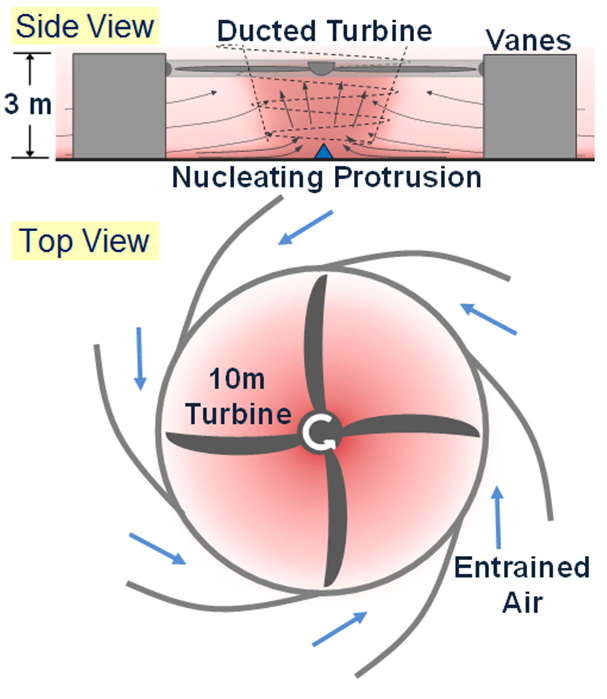
\includegraphics[width=.5\linewidth]{figs/power_generation.png}
   \caption{The Sov facility, showing the vanes, rotor and anchoring
   protrusion, as well as the buoyancy-driven vortex used to drive the
   turbine.}
   \label{facility}
  \end{center}
\end{figure}

The simulations are designed to both mimic the notional SoV experimental
facility as well as identify optimal configurations for future
designs. The general system configuration is depicted in Figure
\ref{facility}. 

Notice several important components of this device. First, ``vanes''
along the sides of the apparatus, designed to entrain outside air and
impart angular momentum. It is not known what configuration and design
of these vanes will lead to optimal dust-devil generation. Thus, these
vanes may have various configurations, varying in the number used, the
length, height, angle of attack. The vanes may also be straight, or
curved.  Next, the ducted turbine above the flow is also a critical design
component. This turbine is designed to extract energy from the flow,
without distrupting/destroying the vortex. Finally, it is desirable to
economically optimize the entire configuration scale by considering both
the power generation, cost of materials, difficulty and expense of
maintainance, etc. 

In addition to the system configuration, it is important to consider the
effect of local conditions on SoV performance. Characterizing the impact
of variations in ambient conditions on the SoV will guide the
commercialization strategy of the product, by determining optimal
install locations across the country. It is therefore desirable to have models
that are capable of accounting for variation in field conditions, such as solar
input, cross-winds and topography. Furthermore, it is expected that 
large ``farms'' of SoVs (akin to the wind and solar farms for wind
turbines 
and photovoltaics, respectively) may be used by commercial or
utility-scale energy generation. In order for this to be effective, 
the inter-unit spacing must also be optimized, as a single SoV collects
from a large area. These computations will guide commercialization
planning, where decision-makers will need to assess optimum unit size,
spacing, and geographic location for utility-scale deployment.  

%
% 2) A complete mathematical specification of the mathematical model
%   (i.e. the equations), with documentation of the basis for the
%   model, what aspects are reliable theory that need not be questioned
%   in the context of this problem, and what aspects are not as
%   reliable (i.e. embedded models), and what is known about how these
%   aspects of the model could be wrong or inaccurate.
%
%
\section{Mathematical Specification}


% navier stokes
We use the 3-D incompressible Navier-Stokes in order to model a
low-speed fluid flow with heat convection and diffusion and buoyancy. 

\begin{align*}
    \bv{R}\left(\left[
    \begin{array}{l}
        \bv{u} \\
        p \\
        T 
    \end{array}
    \right]\right) \equiv& 
    \left[
    \begin{array}{l}
        \frac{\partial (\rho \bv{u})}{\partial t} + \rho \bv{u} \cdot
    \nabla \bv{u} + \nabla p - \mu \nabla^2 \bv{u} + 
    \rho \beta_T (T - T_0) \bv{g} \\
    \nabla \cdot \bv{u} \\
    \frac{\partial (\rho c_p T)}{\partial t} + \rho c_p \bv{u} \cdot
    \nabla T - k \nabla^2 T
    \end{array} 
    \right] = 0
\end{align*}

The Navier-Stokes equations are derived from conservation of mass,
momentum and energy, and are a highly reliable model for low-speed flows
of the sort encountered here. The boussinesq approximation for the
buoyancy is less generally applicable, but still very accurate for a
wide variety of flows in nature, such as atmospheric fronts, oceanic
circulation, etc. The Boussinesq buoyancy approximation relies upon the
difference in density in the fluid being negligible except for gravitational
forces which are large enough to make the specific weight appreciably different
between the two fluids.

Our model also neglects viscous heating. Viscous heating can play an
important role in fluids with strongly temperature-dependent viscosity
because this introduces a coupling between the energy and momentum
equations. This is an important effect in the fluid flow of magma, for
instance.  However, the operating temperatures of our simulations are
sufficiently far from these conditions as to make viscous heating
negligable. 

% embedded models for the vanes!
%An embedded model for the 


%
% 
%3) Identification of all parameters in the model, the available
%   information about these parameters and what is known about their
%   uncertainty.
%
%
\section{Model Parameter Specification}

The most uncertain parameterization in the model comes through the
stabilization parameter. Stabilization is necessary for Finite Element
Methods for fluid flows\cite{franca1992stabilized}. The choice and
design of the stability parameter is a crucial ingredient to ensure the
solution converges. However, the stability parameter also introduces
numerical dissipation, which in addition to altering the solution in a
manner inconsistent with the physical simulation regime, can also
cover-up other discrepancies that might exist in the code. 

Our choice of parameter is guided by a similar numerical
study\cite{Becker2002428} of a incompressible flow with
convection driven by a large temperature. 

However, significant uncertainties still exist. The discretization in
the study only was made with bilinear and biquadratic finite elements. 
While it also used Newton iterations to solve the nonlinear problem, no
time stepping was needed (as the problem was stationary). It is
additionally unclear how the different kinds of discretization and
solvers used in our present simulation may impact the scheme.

%
% 4) Identification of other inputs required for the model (e.g. initial
%   conditions, boundary conditions), and what is known about these
%   inputs for this problem, and associated uncertainties.
%
%
\section{Model Inputs}

The model inputs consistitute a very large component (arguably, the
largest source) of the uncertainty in this problem, for both the
laboratory and outdoor test cases. For brevity, we consider here only
the laboratory cases. 

  \begin{figure}[!htb]
    \begin{center}
     \includegraphics[width = 12 cm]{figs/lab_setup.jpg}
     \caption{The laboratory set-up.}
     \label{lab}
    \end{center}
  \end{figure}

The experimental laboratory has numerous objects
in the immediate vicinity (see figure \ref{lab}) that may
obstruct/manipulate the flow. These objects may be moved or removed
during PIV data gathering. The laboratory simulation uses adiabatic side
walls as a boundary condition. It is unclear how much of an impact this
may have on the simulation. It is also unclear if this is a realistic
boundary condition. 

While no sensitivity analysis has been performed, it is likely that the
largest uncertainty in the laboratory simulation is a result of the
ventilation. This statement can be made because it was observed that the
heated plate on the bottom of the laboratory generated enough heat that
the room temperature began to rise significantly (30+ degrees
Celsius). This also greatly impacted the SoV performance, as the ground
to air thermal gradient drives the vortex. The laboratory uses cooling
in order to maintain temperature. They utilize two inlet HVAC ducts into
the room. While efforts have been made to characterize the level of
ventillation being used, these numbers come with non-trivial
uncertainties attached. As an example, a personal communication with one
of our experimental colleagues, 

``One vent runs continuously at 15 C with a flow rate of about 1
$m^3$/s (4-6 m/s with an approximate area of 0.2 $m^2$).''
Already, the inflow rate has a 50\% uncertainty in velocity
attached. Furthermore, while the area of the vents are given, the the
precise height and width are not. Thus, while our simulation uses square
vents, this may be inaccurate. 
It was also stated that, ``The other vent kicks on only if the
room gets about 28 degrees C.'' This statement has uncertainty attached to the
temperature at which the venting begins. Finally, ``The exit air is just
what ever leaves through/around the doors as we've blocked off all of
the out ducts.'' This also presents a challenge, as it is unclear (for
validation purposes) where one should expect the outflow to
go. \footnote{\normalsize Author note: This story related here not as a comment on
our collaborators. Rather, this is presented as an example of the challenges
and uncertainties that presently exist in this numerical investigation.}

We impose Dirichlet boundary conditions to establish a constant inflow
condition of cool air at the rates proscribed by our
collaborators. Unfortunately, we have found that the using inflow rates
consistent with the lower bound of those estimates result in an
unrealistic heating of the room, while inflow conditions at the high end
result in velocity profiles that exceed the laboratory measurements. In
other words, our simulations appear to be sensitive to the choice of
inflow rate, and it is likely that the laboratory is run where one of
the vents is operating intermittently. 

The initial conditions in both the laboratory and the outdoor
tests are highly uncertain. The dimensions of the laboratory are
(it is presumed) measured with a high degree of confidence, however, the
initial temperature 
in the room is not closely measured, and may vary as a function of
time or across tests. We note however, that the solutions from the simulations are
generally stationary in time, and consistent results are gathered from several
simulations with different initial conditions. Therefore, it does not
appear that the initial conditions in the room in terms of the ambient
velocity or temperature field are a large source of uncertainty in the
laboratory.

%
% 5) A proposal of what (if any) of the parameters/inputs could
% be/should be calibrated, what experimental scenarios could be
% used for this calibration, and whether data is already available,
% or new experiments would be needed. Also describe what, if
% anything, is known about uncertainties in the observational data. 
%

\section{Proposed Model Calibration}

One could, in principle, perform a calibration of some of the model
parameters such as the stabilization coefficient or the boundary
conditions. However, for this particular problem, it is not particularily important to
perform a model calibration. There are several reasons for this. First,
as this is a new modeling regime, the reliability of the data and models
is questionable. As this is a new physical apparatus, very little data
exists at present. The existing data has therefore been
primarily used for validation. While one can certainly
calibrate and validate using the same data, this is not as strong a test 
as a ``blind'' validation using data that a model was not calibrated with. 

Furthermore, as the simulations are expected to be utilized for
extrapolation across a wide range of scenarios and domains, it is
unclear how much use a calibration would be for only one scenario. As
stated previously, the real challenge lies in validation checks that
evaluate the how reliable predictions of the model extrapolate to a wide
range of conditions and situations. 

Finally, our interests are focused on broadly predicting trends and
scaling of the SoV to guide experimental design and testing. Therefore,
it is not, at present, a priority that the model predictions fit the validation
cases extremely tightly, but rather, that the model predictions be
validated in a qualitative manner as quickly as possible, in order to
begin iterating on system designs with our experimental colleagues. 

%
% 6) A proposal of how the model could/should be validated, including
%    validation of any embedded models, as well as the overall model.
%    Identify whether data is already available or whether new
%    experiments would be needed. Also describe what, if anything, is
%    known about uncertainties in the observational data.
%
\section{Model Validation Challenges}


% validation
Several phases of research must be conducted in order to develop robust
and reliable predictive simulation capability. First, the simulations
must be validated against existing experimental data generated from the
laboratory apparatus. These data were taken using particle image
velocimetery (PIV), often not without non-trivial error in measurement and
sampling. Finally, as mentioned previously, the measurements for the
cooling, geometry of the room, etc. are rough, and almost certainly
possess non-trivial uncertainties/errors. As a result, this is already a
difficult validation scenario. 

The validation challenge is compounded by the fact that very little is
known about the uncertainties in the observation data. PIV is a
non-intrusive technique, but it does rely upon large sample sizes in
order to generate reliable statistics. While several hundred PIV
snapshots are available, no quantified uncertainties for the averaged fields
presently exist.  

In addition, only velocity measurements are available. Several
potentially important quantities of interest, such as the pressure field
or the temperature, have not been measured, and cannot then be used for
the purposes of validation. This presents a risk that our 
simulations might generate acceptable velocity fields, but that a
significant source of error may exist in unobserved QoIs, and would not
be detected in our present validation regime. 

Furthermore, the model form in use is known to be imperfect. 
Model inadequacy may play a significant role in both the validation
scenarios described below, as well as (more chillingly) in the
additional regimes that the models will be used in a predictive
capacity. 

%
% first case
%
\subsection{Model Validation}
Our initial focus has therefore moved to a validation study to ensure that the
output of the numerical simulation agrees with the experimental
measurements. The flows are qualitatively similar, with a vortex forming
in the center of in both cases, but the degree to which each matches
each other is unclear and must be characterized. 

\begin{figure}[!htb]
        \centering
        \begin{subfigure}[bh]{0.5\textwidth}
                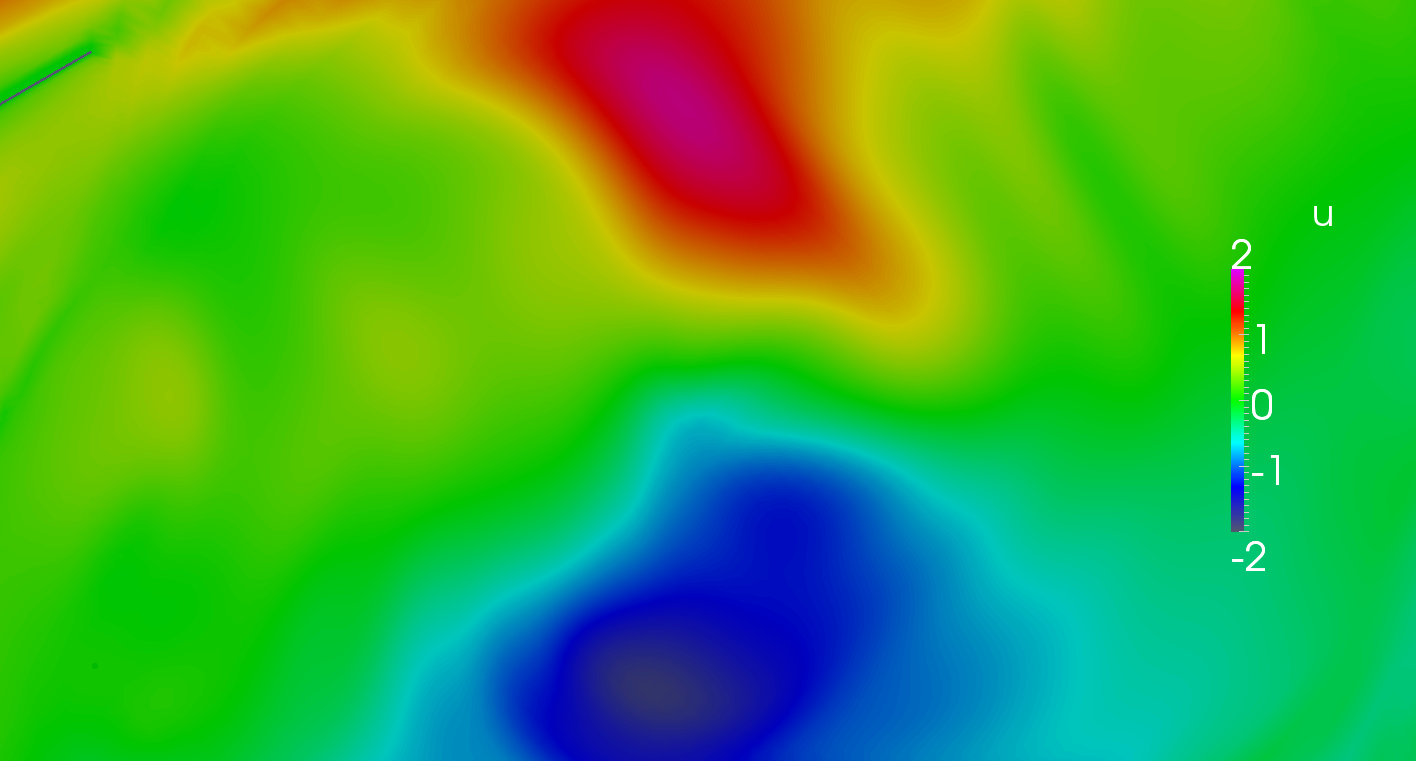
\includegraphics[width=.8\linewidth]{figs/u_sim.png}
        \end{subfigure}%
        \begin{subfigure}[bh]{0.5\textwidth}
                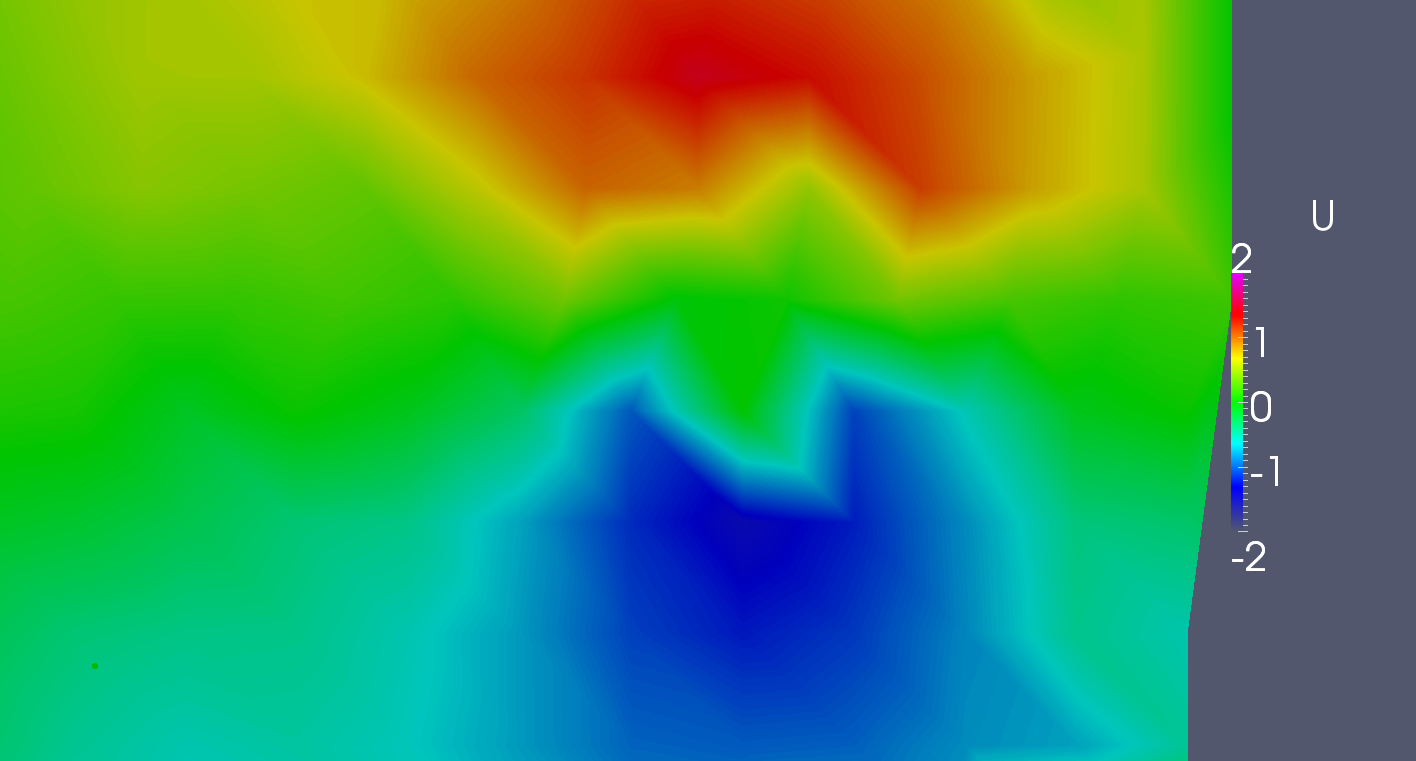
\includegraphics[width=.8\linewidth]{figs/u_exp.png}
        \end{subfigure}
 \caption{The instantaneous x velocity component (u)
 from a horizontal plane situated slightly above the vanes,
 measured in the simulation (left) and the laboratory apparatus
 (right). This is for a 30 degree vane configuration.} 
 \label{fig:instant}
\end{figure}


In particular, we have implemented a simulation designed
to closely mimic the 30 degree vane experimental setup. The outputs of
the simulation (velocity field, temperatures, etc. ) are then compared
to available experimental data, which at this time is principally the
velocity field taken by PIV measurements at a variety of time frames
near the center of the SoV. This ``high-cost'' simulation resolves
the SoV large-scale structure, as well as the turning vanes
nearby. Comparisons must be made between the:
\begin{itemize}
 \item Azimuthal Velocity as a function of radius from center of the Sov
 \item Azimuthal Velocity as a function of the height at different
       points in the SoV
 \item Vertical Velocity as a function of radius from center of the Sov
 \item Vertical Velocity as a function of the height at different
       points in the SoV
\end{itemize}
As noted above, this is an extremely limited set of comparisons. 

%
% hybrid (embedded model)
%
Further validation cases are required. We are now in a position to perform
a validation of the embedded vane model. As described previously, this
uses the same turbulence models, but now without resolving the turning
vanes. Instead of resolving the vanes, for a region in the flow, the
velocity field is forced in a manner similar to as if the fluid was
moving through the turning vanes. While direct comparisons between this
model and the experimental data can be (and will be) made, a comparison between this
``low-cost'' (in terms of computation and mesh requirements) simulation
and is useful for several reasons. It permits directly comparing the effect of
the simple, low cost, turning vane model against the higher resolution
modeling (essentially this permits a validation of an embedded
model). Furthermore, it allows us to observe a much richer set of
possible changes in the state space than in the experiment, which is
constrained to only velocity measurements. 

%
% 7) An assessment of what further concerns might remain after (5) and
%   (6) regarding the applicability of the model for the purpose of the
%   calculations.
%
\section{Further Concerns}

% the fucking turbine too...
Our goal is to eventually extract energy from the SoV, which at this
time is envisioned coming from a turbine placed over the vanes. It will
be very difficult to get accurate PIV measurements from the apparatus in
the laboratory, and once again the simulations will be essential in
driving the experimental optimization and design of the SoV. Thus, 
this adds another significant validation case, with new, significant,
challenges in modeling the turbines. This is in essence a new embedded
submodel that we will add after validation of the initial configuration
is completed. 

In order for these simulations to be generally useful, after they are 
validated against existing experimental data and high fidelity
simulations, they will be used to explore regimes and scales where no
experimental measurements presently exist. Characterizing the
uncertainty of predictions resulting from extrapolation is a critical
component in enabling reliable assessments of field performance of the
SoV, as it will guide the commercialization strategy of the product.

% scaling analysis
These new simulations at different conditions will be performed in order
to inform the optimal design and scale of the planned two and five meter
SoV prototypes, to be installed in Arizona. This study will inform the
design based on the scaling of the velocity field and anticipated energy
generation. Furthermore, insights may be gathered on the dyamics of
these flows, which could lead to fundamental advances in the physics of
fluid dynamics, dust devils, and other coherent structures with vortex 
dynamics\cite{Mullen1977181,smithleslie,kanak}. 

% this might be junk
Determining the optimal design of these systems will involve parameter
sweeps over a large space of possible configurations. These simulatons
are expensive, and so while accuracy is important, where possible,
models will be developed in order to simplify the mesh (memory) and
computational requirements. For instance, the previous ``low-cost'' vane
 method, which replaces the turning
vanes with a model, improved runtime by a factor of twenty-four, due to
the greatly decreased mesh resolution requirements near the vane
trailing edges. These models, if they prove to be robust after
validation testing, will be
invaluable tools in effective computer aided design and simulation of
this new technology.  


%
%
% 8) From this plan, select a sufficiently simplified or constrained
%    sub-problem, on which to formulate the probabilistic analysis of
%    calibration and validation. To the extent possible, symbolically
%    define likelihoods, priors, input uncertainties, data
%    uncertainties, etc., defining probability models for the relevant
%    uncertainties and including things symbolically that you can't
%    specify yet.
%
%
\section{Probabilistic Formulation on a Sub-Problem}


We propose the to calibrate our simuation inflow boundary conditions
against the laboratory data. We will assume that the inflow between the
two HVACs is identical, and that they have the same areas. 

We are therefore inferring three parameters: A (the area of each HVAC), V (the inflow
velocity rate) and T (the inflow temperature). Note that a more rich
model for A might be useful, as $A=b*h$, but for this calibration we
will assume that $A=l^2$, e.g. the area is square. We choose to infer
the velocity and the area seperately (instead of the flow rate, for
instance) because this has important implications for the simulation. In
particular, a higher velocity penetrates deeper into the room more
quickly. 

We are given information that the inflow velocity is $4-6 m/s$. It seems
very unlikely that the velocity cannot be below 4 m/s or higher than 6
m/s. Thus, instead of a uniform distribution, we will use a Gaussian
centered at 5 m/s with the 95\% (two $\sigma$) centered at 4 and 6. 
\begin{equation}
v \sim \mathcal{N}(5,0.5).
\end{equation}

We expect that the area measured to be more accurate, presumably with a
tape-measure or another device with small error (However, the note did
ominously state, ``approximate area''). It seems extremely unlikely this
error is more than 10\%. We therefore set a Gaussian, where again the
95\% (two sigma) range is between 0.08 and 1.2, 
\begin{equation}
A \sim \mathcal{N}(1,0.01).
\end{equation}

The temperature also appears to be uncertain. Here, we have very little
estimate at how much it might be off. It is not known how the 15 degree
C measurement was attained, or if the instrument (one hopes it was not a
hand) was properly calibrated. We therefore choose a broad prior,
with standard deviation of 2 degree centigrade. e.g.
\begin{equation}
T \sim \mathcal{N}(15,2).
\end{equation}

We do not have an estimate for the experimental data uncertainty. Thus,
for the purposes of this calibration, we must necessarily choose a broad
prior that permits room for non-trivial error. However, we note that
aside from the error being zero mean, we do not know much more about the
expected characteristics of it. I'll therefore choose a Gaussian with 10\% (in the
average velocity measured in the PIV) sigma. I am slightly worried this is not
broad enough, however. 
\begin{equation}
\epsilon_d \sim \mathcal{N}(0,.1 \bar w).
\end{equation}

We desire to calibrate our inflow to as closely match the vertical
velocity between the experiment and the simulation as possible. This is
not necessarily because this is our QoI, but because it will have more
implications for power-generation than the azimuthal velocity, and we do
not have access to many quantities to consider. 
\begin{align*}
\pi(w_{\text{fwd model}}=w_{d}\,|\,A,v,T)=\frac{1}{\sqrt{(2\pi)^{n}|.1
 \bar w|}}\exp\left\{ -\frac{1}{2}\left(h_{d}-h^{\text{fwd model}}-\mu\right)^{T}\cdotp\left(h_{d}-h^{\text{fwd model}}-\mu\right)\right\} ,
\end{align*}


%
% end
%
%This work is supported by the Department of Energy [Advanced Research
%Projects Agency-Energy] under Award Number [DE-FOA-0000670].    

\bibliography{references}
\bibliographystyle{unsrt}

\end{document}
